\documentclass{article}
\usepackage[fleqn]{amsmath}
\usepackage{amssymb,graphicx,color,graphicx,slashed, microtype, parskip, enumitem, extarrows, needspace}
%\usepackage[utf8x]{inputenc}
\usepackage[top=1.5cm, bottom=1.5cm, right=6cm, left=1.5cm, heightrounded, marginparwidth=5cm, marginparsep=0.5cm]{geometry}

\hbadness = 10000
\hfuzz=100pt 
    
\usepackage{marginnote}
\renewcommand*{\marginfont}{\footnotesize}

\usepackage{hyperref}
\hypersetup{colorlinks=true, urlcolor=NavyBlue, bookmarksdepth=3}

\makeatletter\newcommand{\@minipagerestore}{\setlength{\parskip}{\medskipamount}}\makeatother

% =============== Index ===========================

\usepackage[nonewpage]{imakeidx}
\makeindex

% =============== Color Definitions ===============
    
\usepackage[svgnames]{xcolor}
\colorlet{ColorTitle}{Black}
\colorlet{ColorSectionName}{Black}
\colorlet{ColorBoxFG}{Gray}
\colorlet{ColorBoxText}{Black}
\colorlet{ColorBoxBG}{White}


% =============== Title Style ===============
    
\usepackage{titling} % Allows custom title configuration
    
\newcommand{\HorRule}{\color{ColorTitle}\rule{\linewidth}{1pt}} % Defines the gold horizontal rule around the title
    
\pretitle{
    \vspace{-50pt} % Move the entire title section up
    \HorRule\vspace{9pt} % Horizontal rule before the title
    \fontsize{27}{36}\usefont{OT1}{phv}{b}{n}\selectfont
    \color{ColorTitle} % Text colour for the title and author(s)
}
    
\posttitle{\par\vskip 15pt} % Whitespace under the title
    
\preauthor{\fontsize{17}{0}\usefont{OT1}{phv}{m}{n}\selectfont\color{ColorTitle}} % Anything that will appear before \author is printed
    
\postauthor{\par\HorRule}

\newcommand{\COURSENAME}{\href{http://phyw.people.ust.hk/teaching/PHYS2022-2015/}{\textcolor{black}{PHYS 2022}}}
\newcommand{\YW}{\href{http://phyw.people.ust.hk/}{\textcolor{black}{Yi Wang}}}
\newcommand{\PHYS}{\href{http://physics.ust.hk}{\textcolor{black}{Department of Physics}}}
\newcommand{\HKUST}{\href{http://www.ust.hk/}{\textcolor{black}{HKUST}}}
\author{\COURSENAME, \YW, \PHYS, \HKUST}

\date{}

% =============== Section Name Style ===============
    
\usepackage{titlesec}
    
\titleformat{\section}
    {\fontsize{15}{20}\usefont{OT1}{phv}{b}{n}\color{ColorSectionName}}
    {\thesection}{1em}{}
    %[{\vspace{0.2cm}\titlerule[0.8pt]}]
    
\titleformat{\subsection}
    {\fontsize{14}{20}\usefont{OT1}{phv}{m}{n}\color{ColorSectionName}}
    {\thesubsection}{1em}{}
    
\titleformat{\subsubsection}
    {\fontsize{12}{20}\usefont{OT1}{phv}{m}{n}\color{ColorSectionName}}
    {}{0em}{}
      
\setcounter{secnumdepth}{4}
        
% =============== Box Style ===============
    
\usepackage[most]{tcolorbox}
    
\newtcolorbox{tbox}[1]{
    colback=ColorBoxBG, colframe=ColorBoxFG, coltext=ColorBoxText,
    sharp corners, enhanced, breakable, parbox=false,
    before skip=1em, after skip=1em,
    title={#1}, fonttitle=\usefont{OT1}{phv}{b}{n}, 
    attach boxed title to top left={yshift=-0.1mm}, boxed title style={sharp corners, colback=ColorBoxFG, left=0.405cm},
    rightrule=-1pt,toprule=-1pt, bottomrule=-1pt
}

\newtcolorbox{mtbox}[1]{
    colback=ColorBoxBG, colframe=ColorBoxFG, coltext=ColorBoxText,
    sharp corners, enhanced, breakable, parbox=false,
    before skip=1em, after skip=1em,
    title={#1}, fonttitle=\usefont{OT1}{phv}{b}{n},
    attach boxed title to top left={yshift=-0.1mm}, boxed title style={sharp corners, colback=ColorBoxFG, left=0.15cm},
    rightrule=-1pt,toprule=-1pt, bottomrule=-1pt, 
    left=0.5em
}

% =============== tikz has to be loaded after xcolor
\usepackage{tikz}

\newcommand*\enumlabel[1]{\tikz[baseline=(char.base)]{
			\node[shape=rectangle,inner sep=2pt,fill=ColorBoxFG] (char) 
			{\fontsize{7}{20}\usefont{OT1}{phv}{b}{n}{\textcolor{ColorBoxBG}{#1}}};}}

% =============== Useful shortcuts ===============

\newcommand\wref[1]{{\hypersetup{linkcolor=white}\ref{#1}}}  

\newcommand{\textbox}[2]{
    \begin{tbox}{#1}
        #2
    \end{tbox}
}

\newcommand{\mtextbox}[2]{\marginnote{
    \begin{mtbox}{#1}
        #2
    \end{mtbox}}
}

\newcommand{\mnewline}{\vspace{0.5em}\newline}

\newcommand{\titem}[1]{
    \begin{itemize}[label=\color{ColorBoxFG}$\blacktriangleright$, leftmargin=0mm, labelsep=0.27cm, topsep=0.5em
        %, itemsep=1ex
        ]
        #1
    \end{itemize}
}

\newcommand{\mtitem}[1]{
    \begin{itemize}[label={\color{ColorBoxFG}$\blacktriangleright$}, leftmargin=0mm, labelsep=1mm, topsep=0.5em
        %, itemsep=1ex
        ]
        #1
    \end{itemize}
}

\newcommand{\itembox}[3]{
    \begin{tbox}{#1}
        #2
        \titem{#3}
    \end{tbox}
}

\newcommand{\mitembox}[3]{
    \marginnote{
    \begin{mtbox}{#1}
        #2
        \mtitem{#3}
	\end{mtbox}
    }
}

\newcommand{\tenum}[1]{
    \begin{enumerate}[label=\protect\enumlabel{\arabic*}, leftmargin=0mm, labelsep=0.265cm, topsep=0.5em
        %, itemsep=1ex
        ]
        #1
    \end{enumerate}
}

\newcommand{\enumbox}[3]{
    \begin{tbox}{#1}
        #2
        \tenum{#3}
    \end{tbox}
}

\newcommand{\twocol}[5]{
    \begin{minipage}[t][][b]
        {#1\textwidth}
        #4        
    \end{minipage}
    \hspace{#2\textwidth}
    \begin{minipage}[t][][b]
        {#3\textwidth}
        #5
    \end{minipage}
}

\newcommand{\cg}[2]{
    \begin{center}
        \includegraphics[width=#1\textwidth]{#2}
    \end{center}
}

\newcommand{\tbar}{
    ~\newline
    {\color{ColorBoxFG}
    \hbox to 0.15\textwidth{\leaders\hbox to 5pt{\hss  \hss}\hfil} 
    \hbox to 0.7\textwidth{\leaders\hbox to 5pt{\hss . \hss}\hfil}}
    \mnewline
}

% =============== Filter unwanted warnings
\usepackage{silence}
\WarningsOff[tcolorbox]
\hbadness=1000000


\graphicspath{{9_fig/}}
\usepackage{ctex}
\title{第九章\ 熵和信息}

\begin{document}

\maketitle

In thermodynamics, you were told by a law that ``entropy'' increases, in order to forbid the dream of a perpetual motion machine. To be more explicit, for an isolated system consists of $n$ subsystems, for each subsystem $i$ define
\begin{align}
    \Delta S_i = \frac{\Delta Q_i}{T} ~,
\end{align} 
where $\Delta Q_i$ is the heat flowing into the subsystem if the process is reversible. Then for a general process, the entropy of the system (Clausius 1855) satisfies the second law of thermodynamics\index{entropy: Clausius}:
\marginnote{And recall that the first law is
\begin{align}\label{eq:tdfirst}
    dE = TdS - pdV~.
\end{align}}
\begin{align}
    \Delta S = \sum_{i=1}^n \Delta S_n \geq 0~.
\end{align}
The equal sign is taken for reversible process; and for non-reversible processes $S>0$. Also, $S$ is a quantity describing the state of the system.

Instead of repeating the standard discussion in thermodynamics here (I assume that you know them. Otherwise see further readings), let us think about a few questions left unclear:

\textbox{The mysterious entropy in thermodynamics}{
    \tenum{
        \item $S$ describes the state of the system. Which aspect of the system does $S$ describe? \marginnote{For other such quantities such as internal energy $E$, volume $V$, pressure $p$, temperature $T$, we can feel them and know what we are talking about.}
        \item Fundamental laws of nature has no arrow of time in it. How can anything increase, which generates an arrow of time?
        \item \label{item:demon} Let's do a thought experiment. \index{Maxwell's demon}
        \marginnote{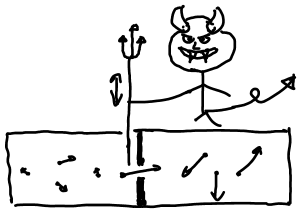
\includegraphics[width=0.3\textwidth]{m_daemon}}
        A box of equilibrium gas is separated into left and right parts, with a small gate in between them. The gate keeper is a little demon (known as Maxwell's demon). The demon only allow molecules with $v>v_0$ to enter the right part and molecules with $v<v_0$ to enter the left part. After some time, would the right part hotter than the left? If so, is the second law of thermodynamics violated?
    }
}



\section{The Statistical Entropy}\label{sec:stat-s}

To take a closer look at entropy, let us first review the condition of equilibrium:

\textbox{Equilibrium of subsystems: thermodynamics}{
    Consider an isolated system containing two sub-systems $A$ and $B$. $A$ and $B$ can exchange heat but each has fixed volume and fixed particle number. The total energy $E=E_A+E_B$ is fixed since the whole system is isolated. Suppose $A$ and $B$ are in thermal equilibrium individually. 
    
    Under which condition is the whole system in equilibrium?
    
    \tcblower

    They have the same temperature. Using the first law \eqref{eq:tdfirst} (with fixed volume and thus $dV=0$), we have
    \begin{align} \label{eq:eq-AB-thermo}
        \frac{dS_A}{dE_A} = \frac{dS_B}{dE_B}~,
    \end{align}
    since both of them equals to $1/T$.
}

\mtextbox{Beyond equal probability}{
    What if we relax our assumption such that each microscopic state has different probability to appear? Then the Boltzmann's entropy formula needs to be generalized. Here we only quote the result:\index{entropy: Gibbs}
    \begin{align}
    S = k_B \sum_i p_i \ln \frac{1}{p_i}~,
    \end{align}
    where the summation runs over all microscopic states. This formula is known as the Gibbs entropy. One can easily check that if for all $i$, $p_i=1/\Omega$, then Gibbs entropy returns to Boltzmann entropy. The Gibbs entropy can be further generalized into the entanglement entropy (Von Neumann entropy) in quantum mechanics.\index{entropy: Von Neumann}
}
\textbox{Equilibrium of subsystems: statistical point of view}{
    Consider the same system as in the previous box. 
    We know the total energy $E$ of the system, and volume and particle number of individual subsystems $A$ and $B$. Given this knowledge, there are exponentially many possible microscopic states \index{microscopic states} satisfying these constraints (these microscopic states as a collection is known as an ensemble\index{ensemble}). 

    We \emph{assume} that each possible microscopic state has equal chance to appear.

    What is the nature of the equilibrium state between subsystems $A$ and $B$? Say, how to partition $E$ into $E_A$ and $E_B$? The partition should correspond to a maximal number of microscopic states, to maximize its probability to appear. 

    For given $E_A$, $E_B=E-E_A$ is fixed. Let's denote the number of possible microscopic states of the subsystem $A$ and $B$ as $\Omega_A(E_A)$ and $\Omega_B(E_B)$, respectively.

    The total number of microscopic states is
    \begin{align}
        \Omega = \Omega_A(E_A) \times \Omega_B(E_B)~.
    \end{align}
    For $\Omega$ to be extremal (most number of microscopic states), we need
    \begin{align}
        0 
        = \frac{d\Omega}{dE_A}  
        = \Omega_B \frac{d\Omega_A}{dE_A} 
        + \Omega_A \frac{d\Omega_B}{dE_B} \frac{dE_B}{dE_A}
        = \Omega_B \frac{d\Omega_A}{dE_A} 
        - \Omega_A \frac{d\Omega_B}{dE_B}~,
    \end{align}
    Thus the equilibrium condition is
    \begin{align}
        \frac{d\ln \Omega_A}{dE_A} = \frac{d\ln \Omega_B}{dE_B}~. 
    \end{align}
    Compared with \eqref{eq:eq-AB-thermo}, we conclude that\index{entropy: Boltzmann}
    \begin{align}
        S = k_B \ln \Omega~,
    \end{align}
    where $k_B$ is a constant, known as the Boltzmann constant. 
    \mtextbox{Entropy and disorder}{
        To be more intuitive about entropy and disorder, consider a box of gas. Each particle can stay either in the left half and right half of the box. An ordered situation is that all particles stay in the left (or right); and a disordered situation is that half particles stay in the left and half stay in the right. There are way more states for the disordered situation. We leave the details to an exercise.
    }    
    Detailed comparison between thermodynamics and statistical physics gives $k_B \simeq 1.38 \times 10^{-23} ~ \mbox{J}/\mbox{K}$. This relation is discovered by Boltzmann in the 1870s and Planck put it into the current form in around 1900.

    \tcblower

    To summarize what we learned here, entropy measure (the logarithm of) the number of possible microscopic states. 
    This can be considered as an indicator of disorder. The 2nd law is thus a more universal saying of ``if you do not clean up your room, it will automatically become more disordered instead of cleaner.''
}

\section{The Arrow of Time}

There is an arrow of time. Time flows toward the future and do not come back. Who has stolen your time? Spilled water take much more efforts to be gathered up again. Who has stolen your efforts?

\textbox{Are past and future equivalent?}{
    In Newton's mechanics of a particle, 
    $ 
      F = m \frac{d^2 x}{dt^2}
    $.
    If we perform the time reversal transformation $t\leftrightarrow -t$, we note that the form of the equation does not change its form. (The action of Newton's mechanics also has the time reversal symmetry).
    
    In fact, for all the known fundamental laws of nature, if we take $t\leftrightarrow -t$, and left to right (parity), and particle to anti-particle (charge conjugate), then nothing changes.
    
    In other words, at the level of a fundamental particle, there is no difference between past and future.
    
    However, we do feel the difference between past and future. Why?    
}

\textbox{Why is there a psychological arrow of time?\index{arrow of time: psychological}}{
    What is the psychological difference between past and future? 
    \marginnote{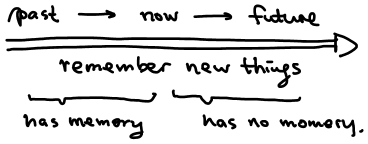
\includegraphics[width=0.35\textwidth]{past_now_future}}
    We remember the things in the past, but not the things in the future.

    Why we can only remember things in the past? Because getting our brain prepared to remembering things needs increase of entropy. Thus the psychological time arrow has to agree with the thermodynamic time arrow, defined by $\Delta S \geq 0$.
}

\mtextbox{(Optional) Entropy and black holes\index{entropy: Bekenstein-Hawking}}{
    Why the earth is spherical? High objects will fall.
    \newline
    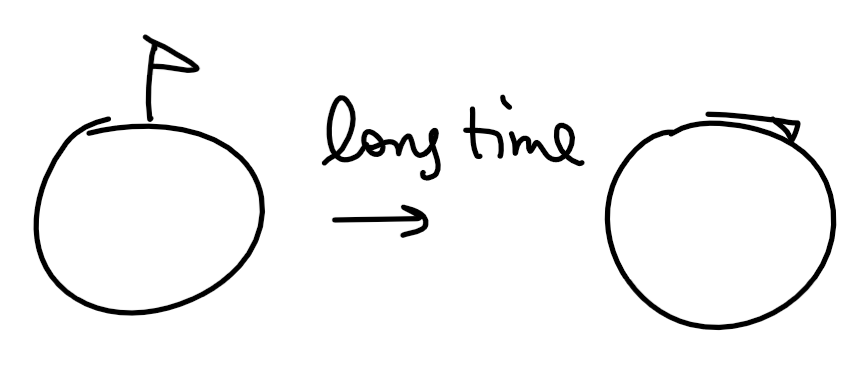
\includegraphics[width=\textwidth]{spherical_flag}
    \newline
    The black hole has infinitely deep gravitational potential. Thus there is no hill on a black hole. Classically, a black hole contains as little information as a fundamental particle: its mass $M$, angular momentum $L$, and charge $Q$. So at first sight, a black hole carries as little entropy as a particle: $S \sim k_B \times O(1)$.
    \tcblower
    Then what if we throw something into the black hole? Would the number of possible microscopic states decrease and thus $\Delta S<0$?
    \mnewline
    Taking quantum mechanics into consideration (Bekenstein \& Hawking), black holes in fact have the hugest number of microscopic states: $S = k_B A / (4l_p^2)$, $l_p \equiv \sqrt{G\hbar/c^3} \simeq 1.6 \times 10^{-35}$m . For example, for a black hole with horizon area $1\mathrm{cm}^2$, the information stored is $10^{65} \sim 2^{216}$, which corresponds to $10^{53}$ hard disks, each with $1$TB capacity. Hard disks are made in the unit of nanometer, while black hole entropy is in the unit of Planck length ($10^{-35}$m).
}
\textbox{Why $\Delta S \geq 0$?}{
    The second law of thermodynamics is somewhat psychological: Even if we live in a universe where entropy decreases, we still feel increase of entropy because we feel that the time arrow is reverted (we can only remember things in the other time direction).
}

\textbox{But why not $\Delta S =0$?\index{arrow of time: thermodynamical}}{
    However, according to statistical physics, a system is more likely in the macroscopic state with maximum underlying microscopic states. If it is the case for our universe, then we should stay in equilibrium almost forever and have $\Delta S = 0$. Why our universe is not the case? Unfortunately, we don't know a definite answer at the moment.
}

\textbox{Other time arrows in physics}{
    There are a few other physical effects which are not time reversal invariant:
    \titem{
        \item The collapse of wave function after measurement. This is probably because of decoherence and follows from the thermodynamics arrow. 
        \item Radiation of charge propagates to the future, not the past. This is again related to the thermodynamic arrow of time. The situation is similar to that we often see a stone drops onto water and water waves propagated away. But we do not often see water waves propagates inward and excite a stone out. (Except in carefully designed devices, for example the Chinese fish basin.)
        \item Black hole (classically) absorbs matter but does not emit matter. It is also related to entropy as we comment in the margin.
        \item Weak interaction. As we mentioned before, we have to revert parity and charge together with time reversal to make weak interaction invariant.
        \item Cosmological expansion. There is no evidence to show that the cosmological expansion is tied to the thermodynamic time arrow. It may be an independent arrow of time.
    }
}

\section{Entropy and Information}\label{sec:info-s}

\textbox{Maxwell's demon\index{Maxwell's demon}}{
    Recall \ref{item:demon} at the beginning of this part: Can the Maxwell demon reduce the entropy? If so, can we use it to do work as a perpetual motion machine? 

    If the demon indeed \emph{knows} the states of the molecules as Maxwell has described, then indeed, he can use it to reduce entropy and do work. As we know,

    \begin{quote}
        Knowledge is power -- Francis Bacon
    \end{quote}

    \tcblower

    Now, does it contradict with the 2nd law? No. Information is not free lunch. There are two possibilities (or combination of them) for the demon to know the states:
    \tenum{
        \item The demon has a huge memory in his brain, to record all the molecule data. In this case, the demon's brain must also contain a huge number of possible configurations $\Omega_D$. The entropy of the demon's brain $S_D=k_B \ln \Omega_D$ must be considered as well. The cost of making the gas from disordered to ordered is to make the demon's brain from ordered to disordered. 
        \item The demon has little (say, only one bit of) memory. So he has to measure and know the information about the molecules one by one when they arrive. To know the state of one molecule, the demon has to erease the state of the previous molecule from his mind. Landauer (1961)\index{Landauer's principle} noticed that, to erase one bit of information, the minimal entropy generated is $k_B \ln 2$ (from the 1st law, the associated heat is at least $k_B T \ln 2$). Adding this part of increased entropy, the 2nd law is not broken.
    }
}

The Maxwell's demon unveils deep connection between entropy and information. What's information?

\textbox{From a newspaper editor to an information theorist\index{information content}}{
    Journalists may be among the first people who understand information deeply. They benefit from news (information). What is a piece of news (information)?

    For example, in 1909, a newspaper editor Greeley said,
    \begin{quote}
        If a dog bites a man that's nothing; but if a man bites a dog, that's news.
    \end{quote}
    Following the spirit of Greeley, what's two pieces of news (information)? Two men bites two dogs, respectively and independently, are two pieces of news.
    \tcblower
    What can we observe about the nature of information from above?
    \titem{
        \item A man bites a dog is more informative than a dog bits a man: for an event with probability $p$ to happen, the information content $h(p)$ should be a decreasing function of $p$. For example, $h(p)$ may be related to $1/p$ in some ways.
        \item Two men bites two dogs are two pieces of information: Information is additive for the information content of independent events. For two events with $p_1$ and $p_2$ probabilities to happen, the probability for both of them to happen is $p_1 p_2$. Thus the informaiton content should satisfy
        $ h(p_1p_2) = h(p_1) + h(p_2) $.
    }
    The most natural function to satisfy the above observations is \marginnote{Here we have used logarithm of base 2 just to match the convention of information theory. It's trivial to convert it to physicists convention by noting $\log_2 x = \ln x / \ln 2$.}
    \begin{align}
        h(p) = \log_2 \frac{1}{p} ~.
    \end{align}

    The unit of information content is \emph{bit}, since it reflects the minimal binary bits needed to encode the corresponding information.
}

\textbox{\emph{Thought experiment}: efficient cheating in an exam}{
    Let's do a thought experiment, i.e. don't do it in reality: cheat in an exam with your partner, by sending answers of multiple choice questions (one of $A$, $B$, $C$, $D$) by binary code. You would like to send minimal length of binary codes to minimize the chance of being caught. Suppose you know the probability $p_A, p_B, p_C, p_D$, how to encode the cheat message most efficiently?

    Instead of a general discussion, let's consider two examples:
    \tenum{
        \item $p_A=p_B=p_C=p_D=1/4$. The information conetent for each choice is $\log_2 (4) = 2$. In other words, each piece of information deserves two binary bits of information. We may encode like $A\rightarrow 00$, $B\rightarrow 01$, $C\rightarrow 10$, $D\rightarrow 11$.
        \item $p_A=1/8$, $p_B=1/8$, $p_C=1/2$, $p_D=1/4$. This is more interesting. A naive cheater may still use two bits to send each choice. But is it the most efficient?
        
        It is intuitive to note that $C$ is more likely to appear, and thus it deserves a shorter code. $A$ and $B$ are rare so we can bear with longer codes. Formally, we can compute: $h(A)=3$, $h(B)=3$, $h(C)=1$, $h(D)=2$. That suggests
        \marginnote{This encoding can be done easily using a \href{https://en.wikipedia.org/wiki/Huffman_coding}{Huffman encoder}. \href{https://planetcalc.com/2481/}{Online calculators} are available.}
        that we can encode like $A \rightarrow 000$, $B \rightarrow 001$, $C\rightarrow 1$, $D\rightarrow 01$. This is known as the Huffman encoding.
    }
    \tcblower
    Let us now verify that the Huffman encoding is indeed more efficient. To do so, we compute the \emph{average information content}, i.e. average length of binary code for sending one answer:
    \begin{align}
        \left \langle h \right \rangle = \sum_{i=A,B,C,D} p_i h(i) = \sum_{i=A,B,C,D} p_i \log_2 \frac{1}{p_i}  = 1.75~.
    \end{align}
    This is indeed shorter than that of the fixed length coding (2 binary numbers per answer). Shannon's source coding theorem says that you cannot get any better. This is why lossless compression (something like zip, rar, 7z in your computer with smaller file size than original) is possible.

    Have you found the equation above similar to something we have learned in physics?
}

\textbox{Information entropy\index{entropy: Shannon}}{
    Inspired by the above discussion, the information entropy is defined as the weighted average information content for all possible outcomes. If we have a set of events $X$, each event $i\in X$ has a probability $p_i$ to happen, then the entropy is
    \begin{align}
      H(X) = \sum_{i\in X} p_i \log_2 \frac{1}{p_i}~. 
    \end{align}
    $H(X)$ is known as the Shannon entropy (Shannon 1948). Again, it has the same meaning as the average information content. 
    \tcblower
    Back to physics, up to a constant, the information entropy is nothing but the Gibbs entropy:       
    \begin{align}
        S = (k_B \ln 2) \times H~,
    \end{align} 
    where the $p_i$ in the definition of $H$ is now restricted to physical microscopic states. 
}

\section{Epilogue: Summary and What's Next}

\textbox{Further reading about the content}{
    \titem{
        \item For statistical mechanics, find a textbook to find more. For example, \href{https://www.amazon.com/Statistical-Mechanics-Third-R-Pathria/dp/0123821886}{``Statistical Mechanics''}, Pathria and Beale.
        \item For black hole entropy, read \href{https://www.amazon.com/Black-Hole-War-Stephen-Mechanics/dp/0316016411}{``The Black Hole War''}, Susskind.
        \item For information theory, read Shannon's paper: \href{http://math.harvard.edu/~ctm/home/text/others/shannon/entropy/entropy.pdf}{``A Mathematical Theory of Communication''}.
        \item For connection between information theory and statistical physics, read \href{https://arxiv.org/abs/0708.2837}{``The Physics of Information''}, Bais and Farmer.
    }
}

\textbox{What happens next?}{
    Statistical mechanics will be the next course to learn for understanding entropy, thermodynamics and much more based on the microscopic states of the system. There is another course of information physics. And definitely information theory is a corner stone of computer science and modern communication. There are many related courses in the School of Engineering.
}

\section{Exercises}

\textbox{E\wref{sec:stat-s}-1 Count the number of states in a simple system}{
    Consider gas in a box (classically without involving quantum mechanics) containing $N$ distinguishable molecules. Let us coarse-grain the state of each molecule as being in the left half and the right half of the box. Then each molecule has two states: $L$ or $R$. Compute the number of states with $M$ molecule in the left half and $N-M$ molecules in the right half. Find the entropy of such state and find the maximal entropy state when varying $M$.
}

\textbox{E\wref{sec:info-s}-1 Find the different object using a balance}{
    Given 12 balls, one and only one of them has different weight. With a balance, how to use fewest measures to make sure to find out the different one?
    \tcblower
    Hint: for the first measurement, one can calculate the information content and entropy of all possibilities and choose the measurement method with maximal entropy. Then the second measurement, etc.
}

\printindex

\end{document}
